\documentclass{article}

\usepackage{amsmath}
\usepackage{amssymb}
\usepackage{xcolor}
\usepackage{tikz}
\usepackage[shortlabels]{enumitem}
\usepackage{float}
\usepackage{wrapfig}

\usepackage[utf8]{inputenc}
\usepackage[T1]{fontenc}

\usepackage[polish]{babel}

\usepackage{listings}
\lstset{
    language=SQL,
    inputencoding=utf8x,
    extendedchars=\true,
    literate={ą}{{\k{a}}}1
             {Ą}{{\k{A}}}1
             {ę}{{\k{e}}}1
             {Ę}{{\k{E}}}1
             {ó}{{\'o}}1
             {Ó}{{\'O}}1
             {ś}{{\'s}}1
             {Ś}{{\'S}}1
             {ł}{{\l{}}}1
             {Ł}{{\L{}}}1
             {ż}{{\.z}}1
             {Ż}{{\.Z}}1
             {ź}{{\'z}}1
             {Ź}{{\'Z}}1
             {ć}{{\'c}}1
             {Ć}{{\'C}}1
             {ń}{{\'n}}1
             {Ń}{{\'N}}1
}

\title{Formy kwadratowe}
%\author{You}

\begin{document}
\maketitle

\begin{enumerate}

\item Podać macierz $A = A^{T}$ powiązaną z formą kwadratową:
    \begin{enumerate}[a)]
        \item $F(x, y) = x^2 + y^2$,
        \item $F(x, y) = x^2 + 2xy + y^2$,
        \item $F(x, y) = -x^2 + xy + 2y^2$,
        \item $F(x, y) = x^2 - 4xy + y^2$,
        \item $F(x, y) = x^2$,
        \item $F(x, y) = -y^2$,
        \item $F(x, y) = x^2 - y^2$.
    \end{enumerate}

\item Naszkicować wykres formy kwadratowej:
    \begin{enumerate}[a)]
        \item $F(x, y) = x^2 + y^2$,
        \item $F(x, y) = x^2 + 2xy + y^2$,
        \item $F(x, y) = x^2 + \frac{1}{2}xy + y^2$,
        \item $F(x, y) = x^2 - 4xy + y^2$,
        \item $F(x, y) = x^2$,
        \item $F(x, y) = x^2 - y^2$.
    \end{enumerate}

\item Sprowadzić formę kwadratową do postaci kanonicznej:
    \begin{enumerate}[a)]
        \item $F(x, y) = x^2 + 2xy + y^2$,
        \item $F(x, y) = x^2 - 4xy + y^2$,
        \item $F(x, y, z) = -x^{2} + 2xy + y^{2} -4yz$.
    \end{enumerate}

\item Sprawdzić określoność formy kwadratowej:
    \begin{enumerate}[a)]
        \item $F(x, y) = x^2 + 3xy + y^2$,
        \item $F(x, y, z) = x^2 + y^2 + 2xy + 4xz + 2yz$,
        \item $F(x, y, z) = -x^{2} - 2y^{2} - 5z^{2} - 2xy - 4yz$,
        \item $F(x, y, z) = x^{2} + 2y^{2} + 5z^{2} + 2xy - 2xz$.
    \end{enumerate}
    
\item Dla jakich wartości parametru $\alpha \in \mathbb{R}$ zachodzi $F(x, y, x) > G(x, y, z)$ dla $\mathbb{R}^{3} - \{ [0, 0, 0] \}$
gdy:
    \begin{itemize}
        \item $F(x, y, z) = 5x^{2} + y^{2}  + 2\alpha xz + 2xy$,
        \item $G(x, y, z) = x^{2} - y^{2}  - 2xy - z^{2}$.
    \end{itemize} 

\end{enumerate}
    

\newpage
\textbf{Odpowiedzi:}
\begin{description}
    \item [1:] a) $A = \begin{bmatrix}\begin{array}{rr} 1 & 0 \\ 0 & 1 \end{array}\end{bmatrix}$,
    b) $A = \begin{bmatrix}\begin{array}{rr} 1 & 1 \\ 1 & 1 \end{array}\end{bmatrix}$,
    c) $A = \begin{bmatrix}\begin{array}{rr} -1 & \frac{1}{1} \\ \frac{1}{1} & 2 \end{array}\end{bmatrix}$,
    d) $A = \begin{bmatrix}\begin{array}{rr} 1 & -2 \\ -2 & 1 \end{array}\end{bmatrix}$,
    e) $A = \begin{bmatrix}\begin{array}{rr} 1 & 0 \\ 0 & 0 \end{array}\end{bmatrix}$,
    f) $A = \begin{bmatrix}\begin{array}{rr} 0 & 0 \\ 0 & -1 \end{array}\end{bmatrix}$,
    g) $A = \begin{bmatrix}\begin{array}{rr} 1 & 0 \\ 0 & -1 \end{array}\end{bmatrix}$,

    \item [2:] a) b) c) d) e) f)
    \begin{figure}[H]
        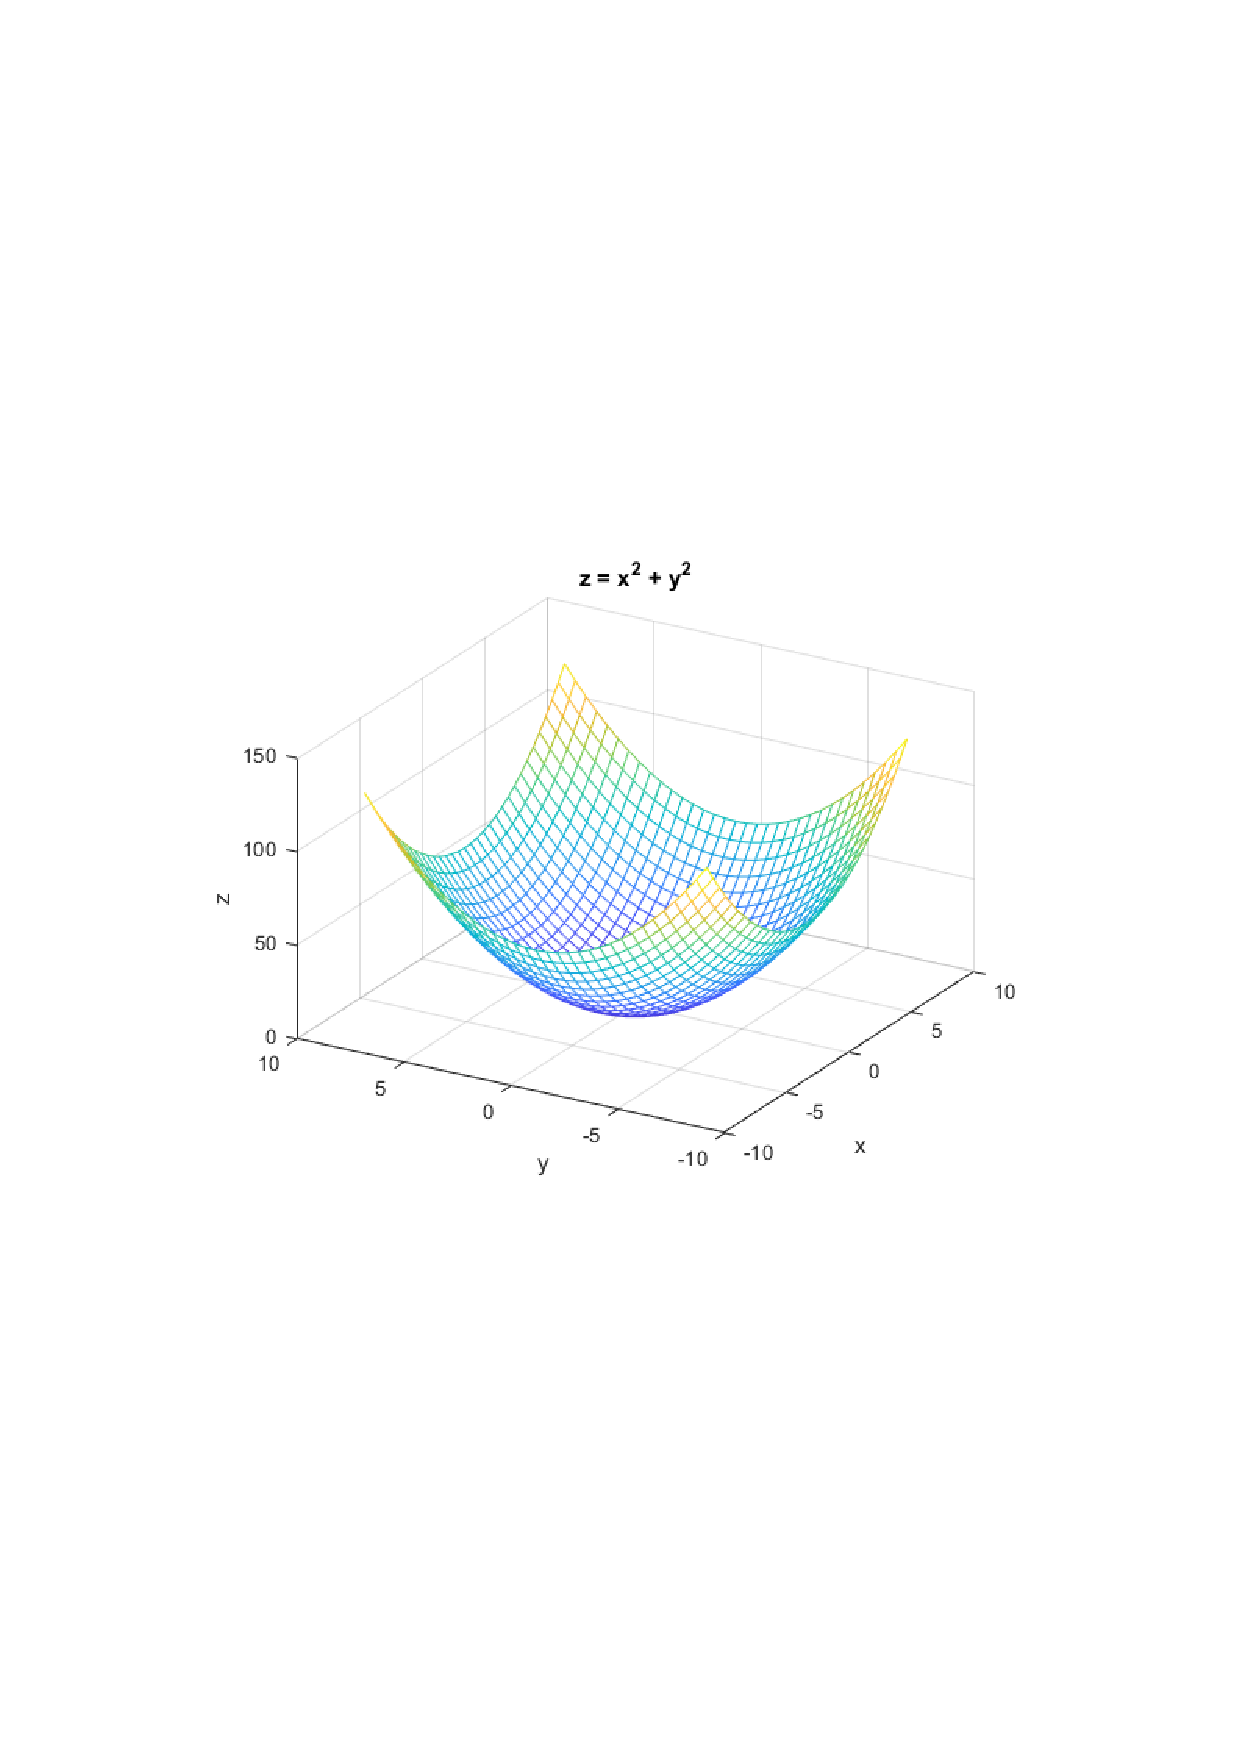
\includegraphics[width=.4\textwidth]{fig/fk_1.pdf}\hfill
        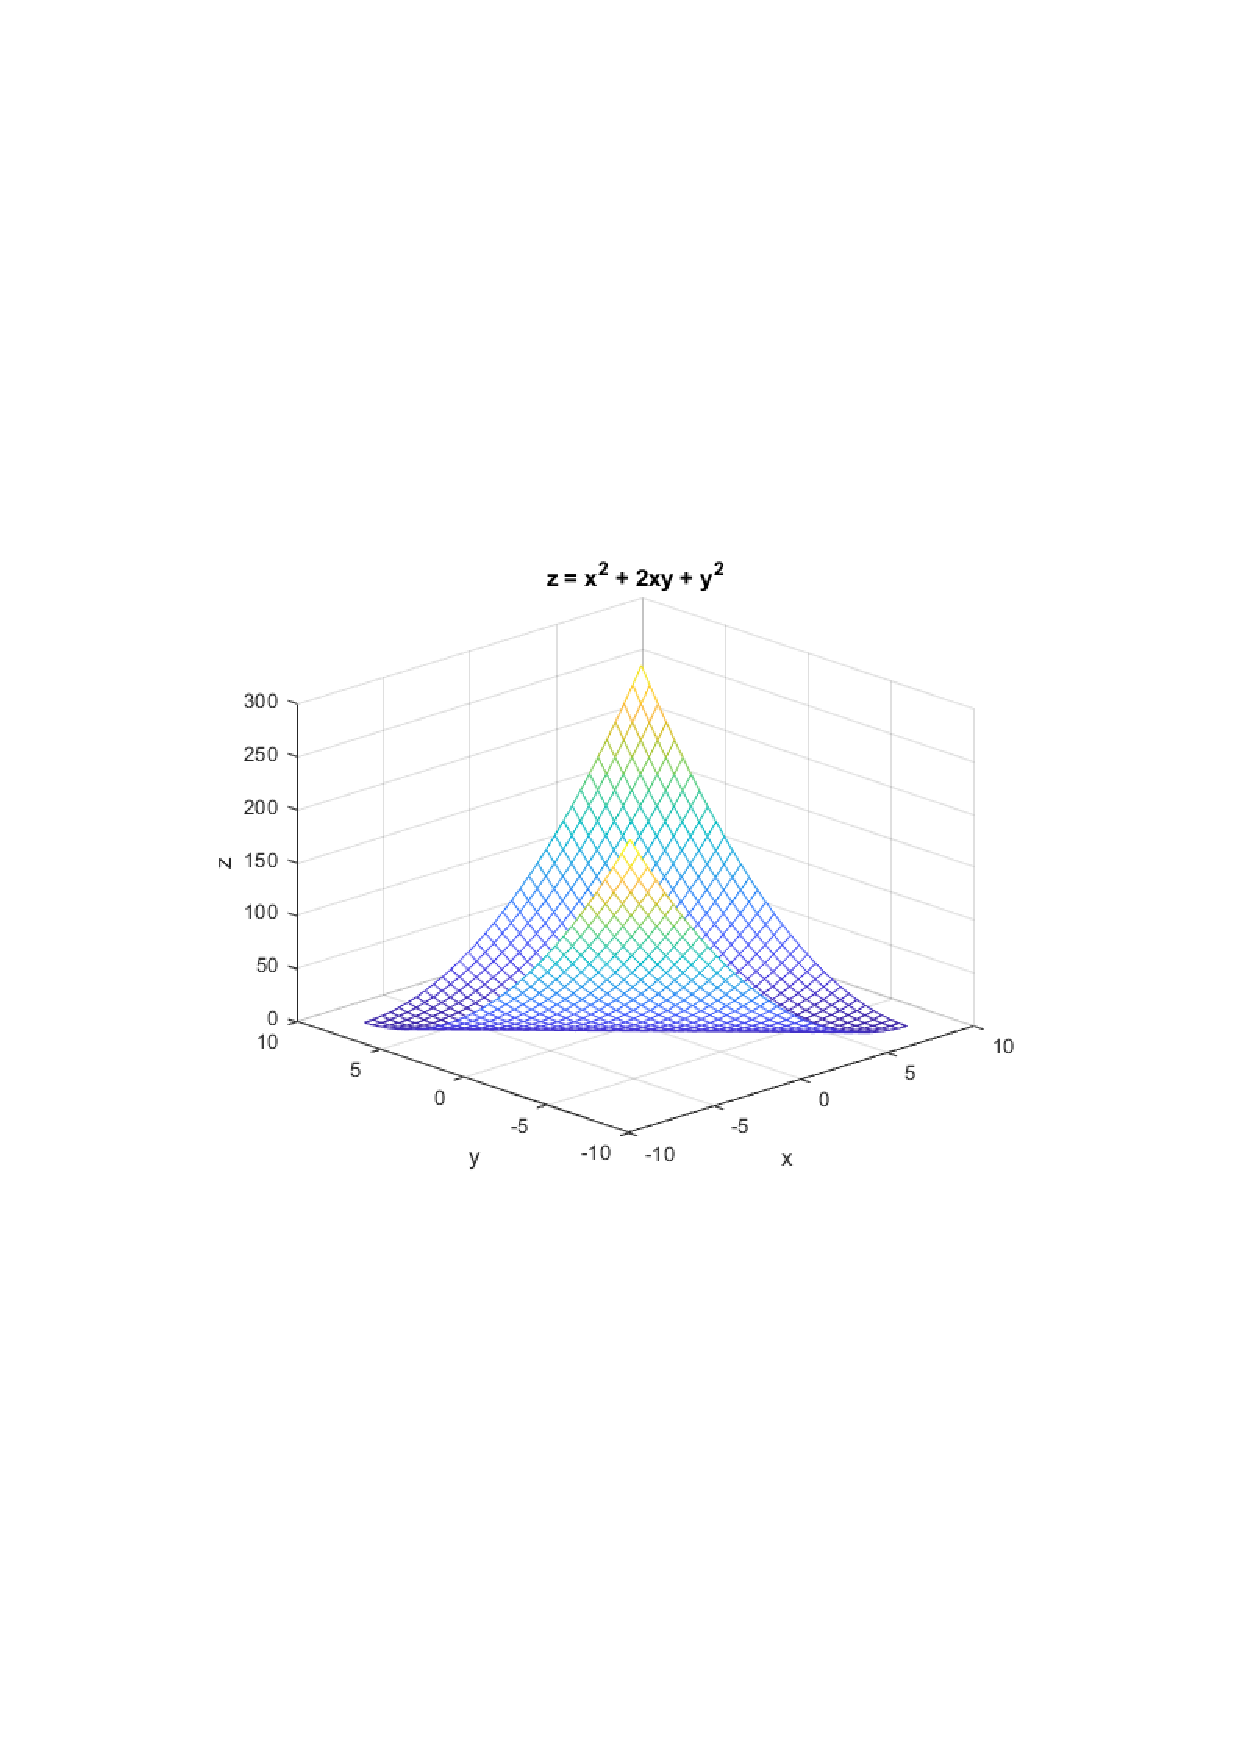
\includegraphics[width=.4\textwidth]{fig/fk_2.pdf}\hfill
        \\[\smallskipamount]
        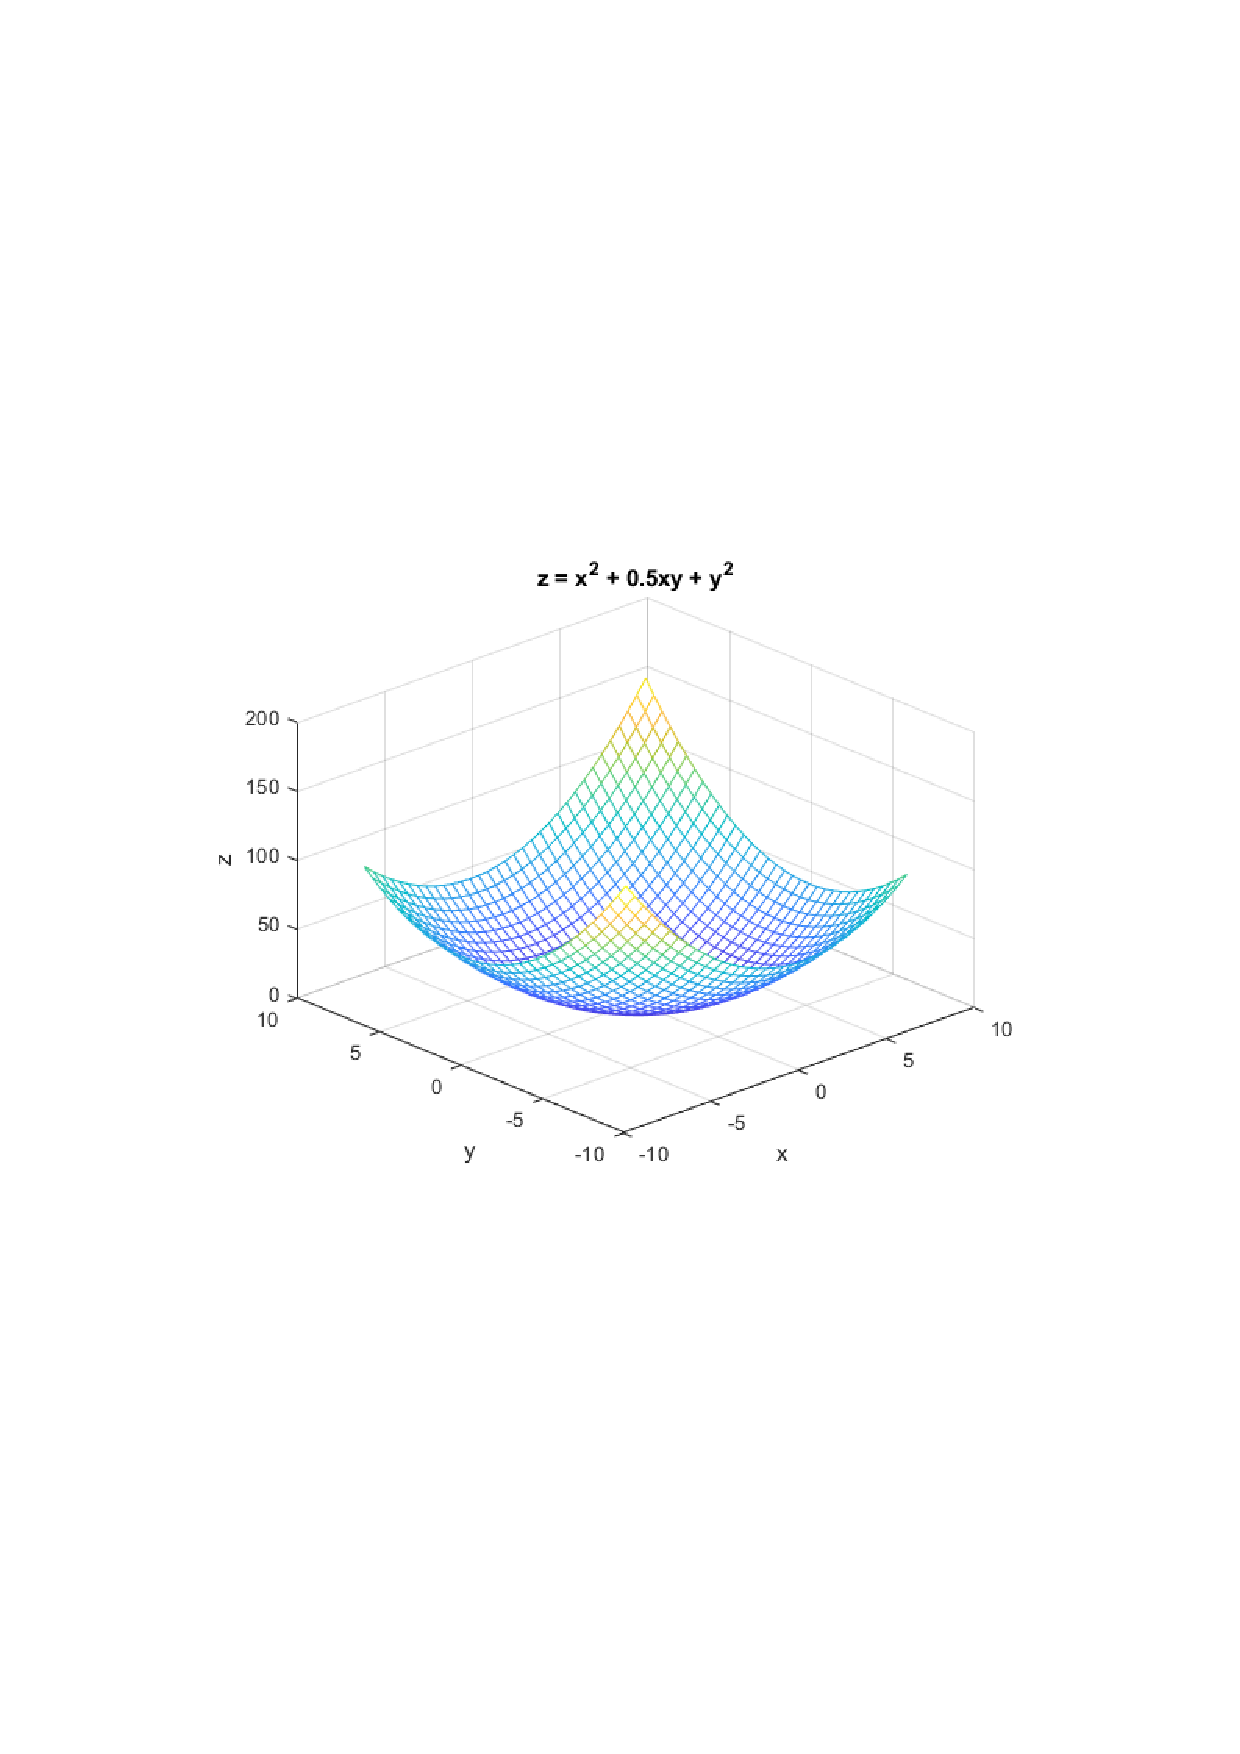
\includegraphics[width=.4\textwidth]{fig/fk_3.pdf}\hfill
        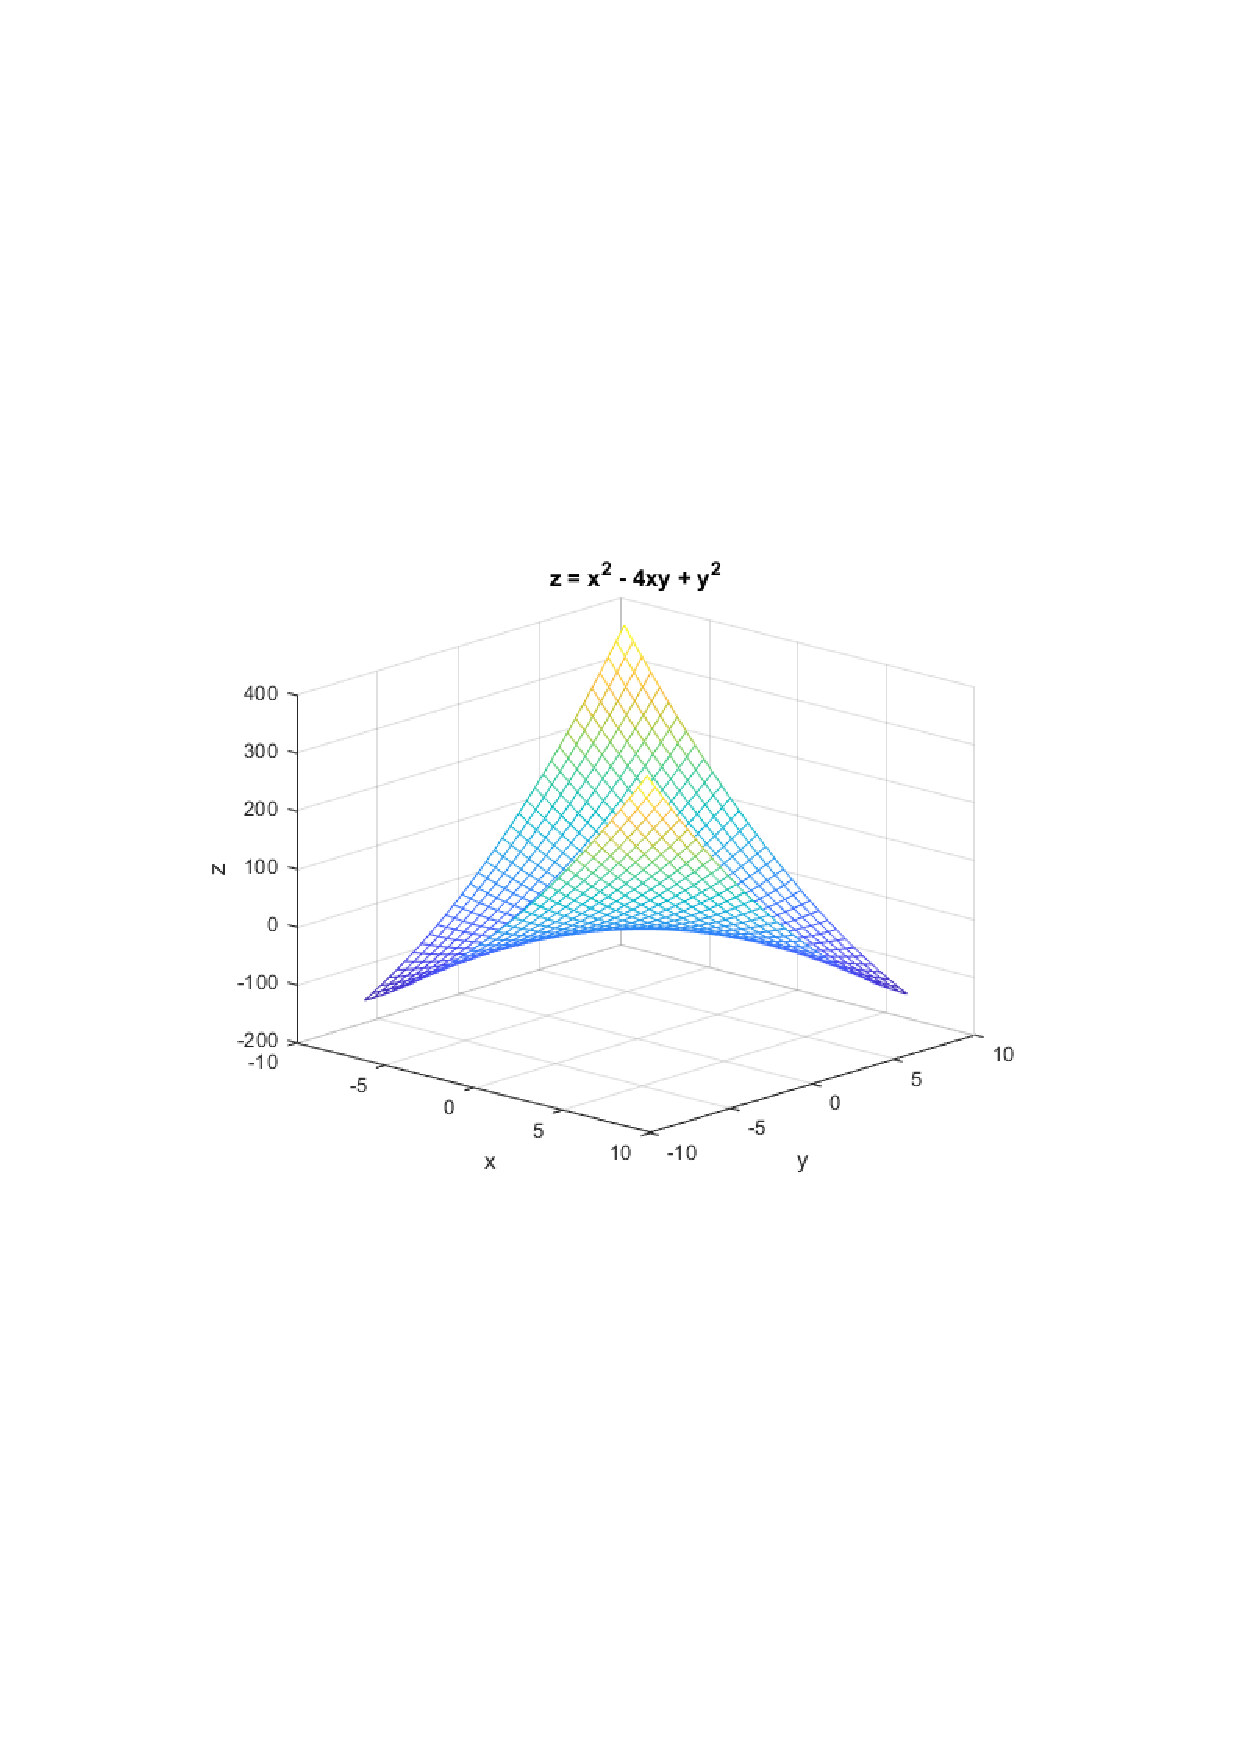
\includegraphics[width=.4\textwidth]{fig/fk_4.pdf}\hfill
        \\[\smallskipamount]
        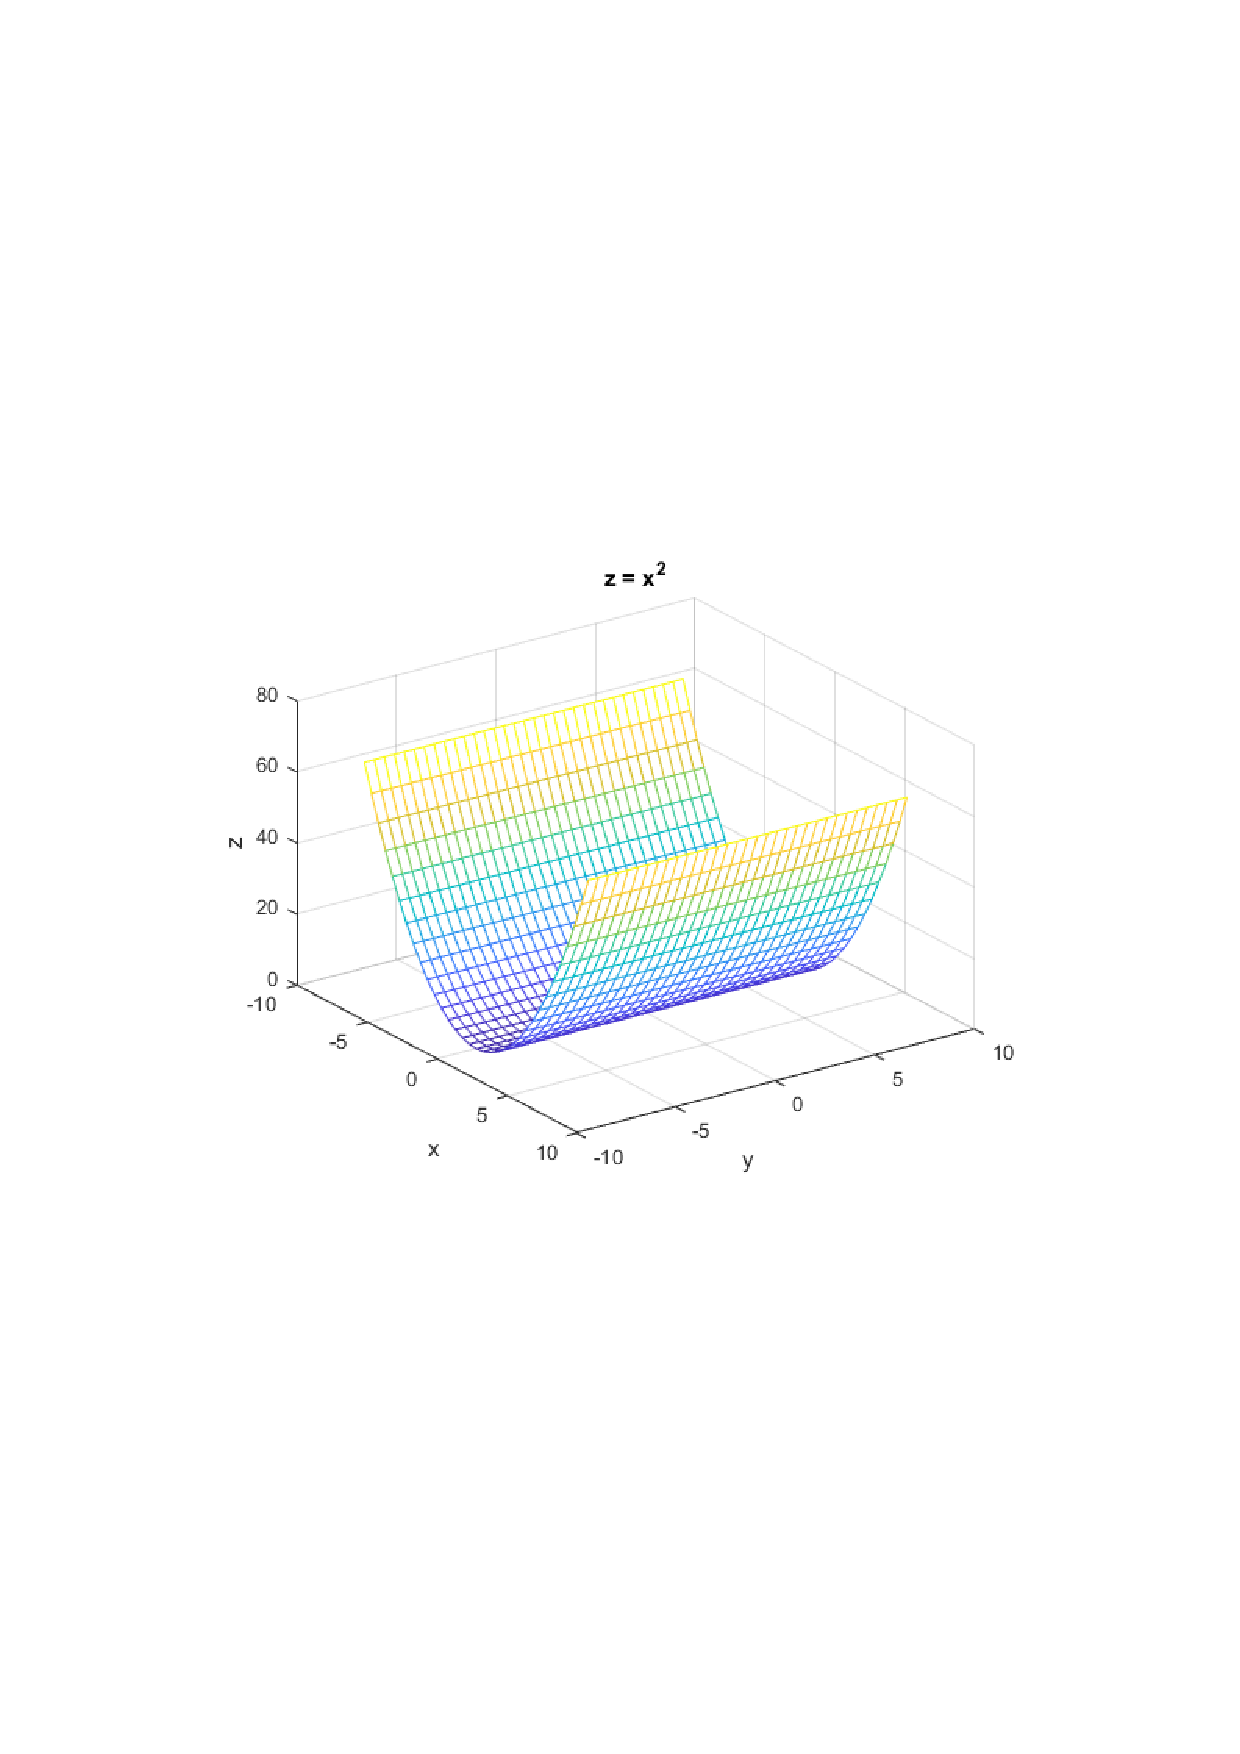
\includegraphics[width=.4\textwidth]{fig/fk_5.pdf}\hfill
        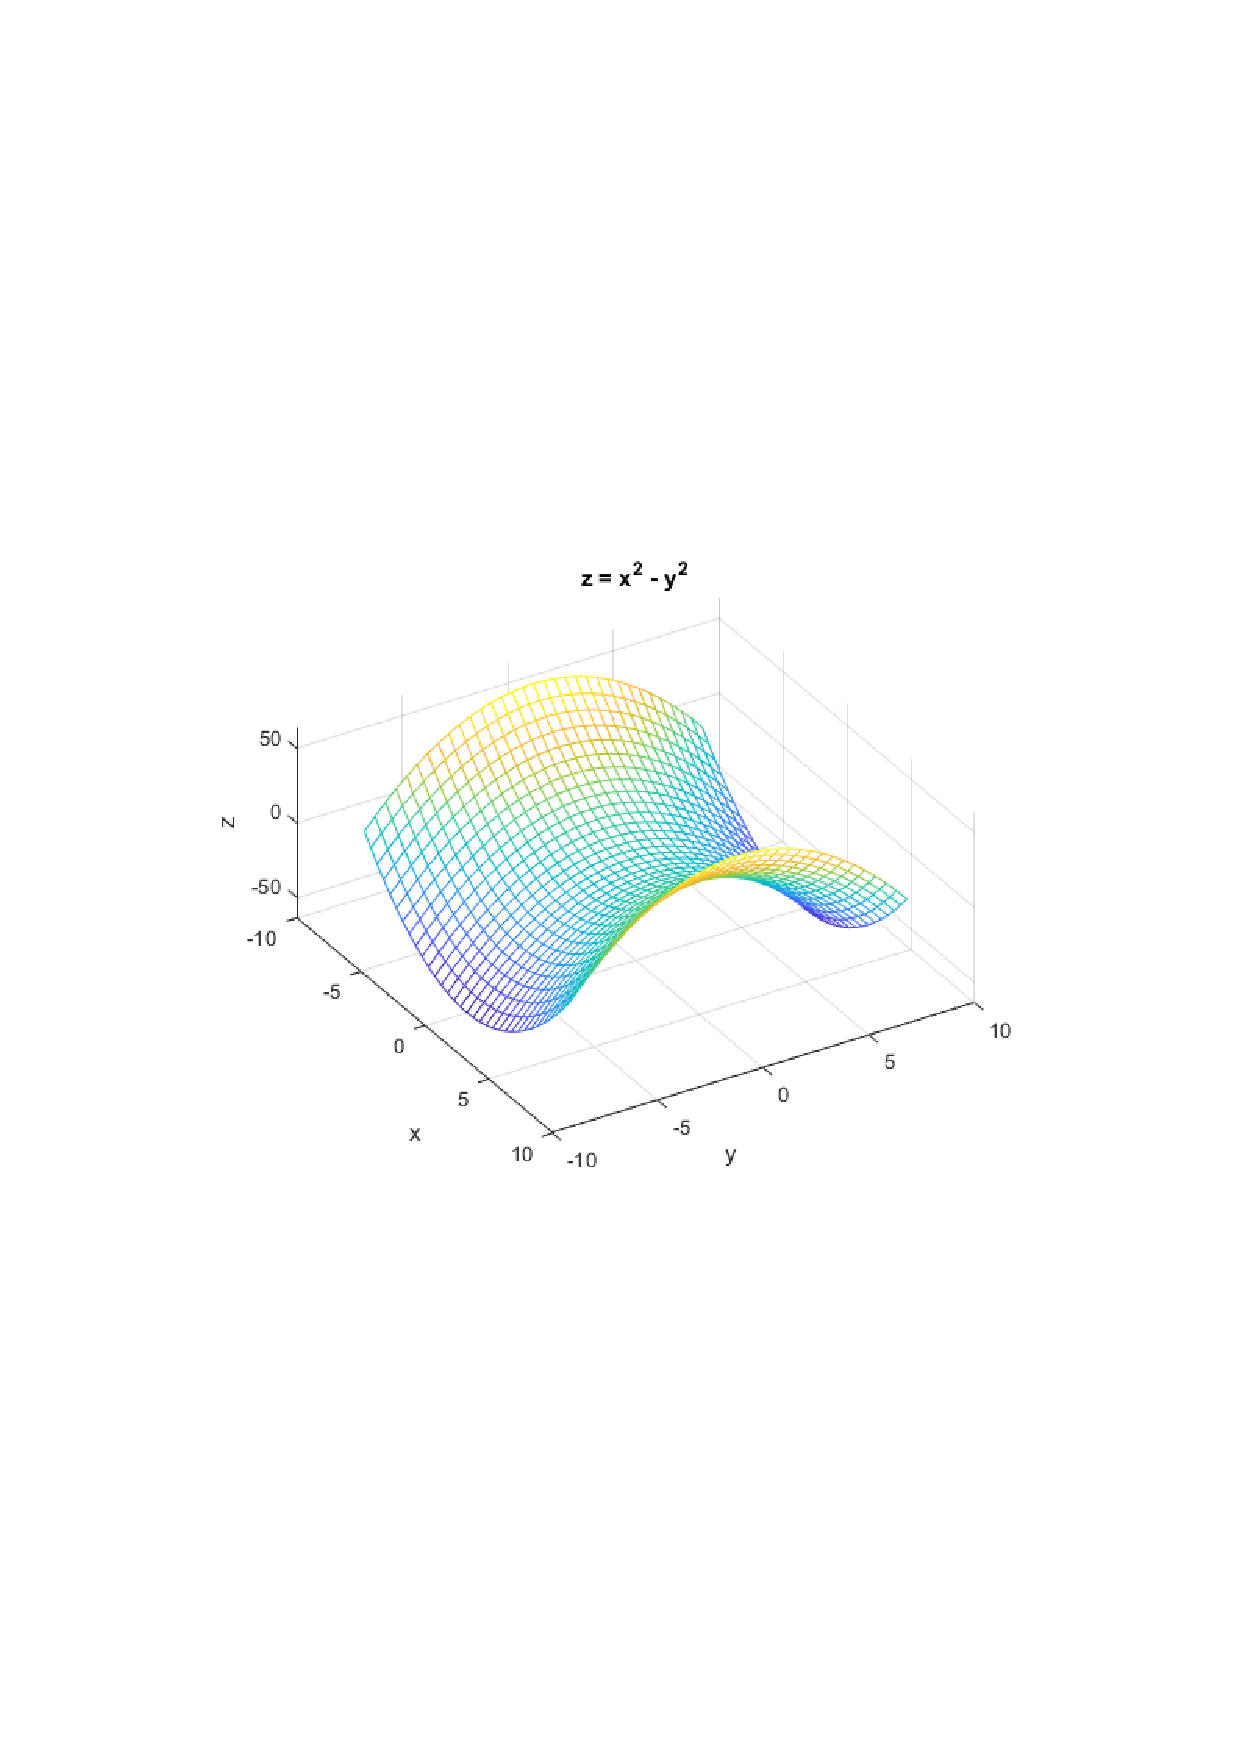
\includegraphics[width=.4\textwidth]{fig/fk_6.pdf}
    \end{figure}

    \item [3:] a) $F(a, b) = a^2$, $P = \begin{bmatrix}\begin{array}{rr} 1 & -1 \\ 0 & 1 \end{array}\end{bmatrix}$,
    b) $F(a, b) = a^2 - 3b^{2}$, $P = \begin{bmatrix}\begin{array}{rr} 1 & 2 \\ 0 & 1 \end{array}\end{bmatrix}$
    b) $F(a, b, c) = -a^2 + 2b^{2} - 2c^{2}$, $P = \begin{bmatrix}\begin{array}{rrr} 1 & 1 & 1 \\ 0 & 1 & 1 \\ 0 & 0 & 1 \end{array}\end{bmatrix}$
    
    \item [4:] a) Nieokreślona, b) Nieokreślona, c) Ściśle ujemnie określona, d) Ściśle dodatnio określona
    
    \item [5:] $\alpha \in (-\sqrt{2}, \sqrt{2})$ 
\end{description}

\end{document}